\subsection{Isotropy groups of a cohomotoper}

Let G and H be groupoids and let \(\varphi\) , \(\psi\) be groupoid morphisms from H to G. The purpose of this section is to compute the isotropy groups of the cohomotoper \(\mathrm{Coh}(\varphi, \psi)\). We retain the notation \(G_1, h_1, \theta_1, \alpha, h\) of No. 3.

Denote by \(\Gamma_{0}\) the frame of the pair \((\varphi,\psi)\). Recall (II, p. 185, def. 3) that this is the quiver \((\mathrm{Orb}(\mathrm{G}),\mathrm{Orb}(\mathrm{H}),\varphi_{0},\psi_{0})\) , where \(\varphi_{0}\) and \(\psi_{0}\) are the maps from \(\mathrm{Orb}(\mathrm{H})\) to \(\mathrm{Orb}(\mathrm{G})\) induced by the maps \(\varphi\) and \(\psi\) by passage to orbits.

Throughout the rest of this section, we will further assume that the quiver \(\Gamma_{0}\) is connected and nonempty; by II, p. 185, prop. 4, this amounts to assuming that the groupoid \(\mathrm{Coh}(\varphi,\psi)\) is transitive, or equivalently that the quiver \(G_{1}\) is connected and nonempty (II, p. 185, prop. 2).

DEFINITION 4. --- We call base equipment of the pair \((\varphi, \psi)\) the data:

\begin{enumerate}
\def\labelenumi{(\roman{enumi})}
\item
  For every \(i \in \mathrm{Orb}(\mathbf{G})\), a vertex \(a(i)\) in the orbit \(i\) of \(\mathbf{G}\) ;
\item
  For every \(j \in \mathrm{Orb}(\mathrm{H})\), a vertex \(b(j)\) in the orbit \(j\) of H;
\item
  For every \(j \in \text{Orb(H)}\), arrows \(c_{1}(j)\) and \(c_{2}(j)\) in G connecting respectively \(\varphi(b(j))\) to \(a(\varphi_{0}(j))\) and \(\psi(b(j))\) to \(a(\psi_{0}(j))\) ;
\item
  A subquiver T of the frame \(\Gamma_{0}\) whose associated graph is a maximal tree of the graph \(\widetilde{\Gamma}_{0}\) ;
\item
  An orbit \(i_{0}\) of G.
\end{enumerate}

Let us choose a base equipment \((a,b,c_{1},c_{2},\mathrm{T},i_{0})\) of the pair \((\varphi,\psi)\). We define a quiver morphism \(\tau_{1}\) from \(\Gamma_{0}\) to \(\operatorname{Grp}(\mathrm{G}_{1})\) by setting \(\tau_{1}(i)=a(i)\) for \(i\in\operatorname{Som}(\Gamma_{0})=\operatorname{Orb}(\mathrm{G})\) and

\[
\tau_ {1} (j) = c _ {1} (j) ^ {- 1} \cdot h _ {1} (b (j)) \cdot c _ {2} (j)
\]

for \(j \in \mathrm{Fl}(\Gamma_{0}) = \mathrm{Orb}(\mathrm{H})\). We shall denote by \(\tau_{0}\) the composite of \(\tau_{1}\) and the canonical morphism \(\theta_{1}\) from \(\mathrm{Grp}(\mathrm{G}_{1})\) to \(\mathrm{Coh}(\varphi, \psi)\) ; it is a quiver morphism from \(\Gamma_{0}\) to \(\mathrm{Coh}(\varphi, \psi)\) .

For \(i \in \mathrm{Orb}(\mathrm{G})\) , denote by \(\alpha_i \colon \mathrm{G}_{a(i)} \to \mathrm{Coh}(\varphi, \psi)_{a(i)}\) the group homomorphism deduced from the morphism \(\alpha \colon \mathrm{G} \to \mathrm{Coh}(\varphi, \psi)\) by restriction to the isotropy groups at \(a(i)\) .

For \(j\in \mathrm{Orb(H)}\) , denote by

\[
\varphi_ {j} = \mathrm{Int} (c _ {1} (j)) ^ {- 1} \circ \varphi_ {b (j)} \colon \mathrm{H} _ {b (j)} \to \mathrm{G} _ {a (\varphi_ {0} (j))}
\]

and

\[
\psi_ {j} = \mathrm{Int} (c _ {2} (j)) ^ {- 1} \circ \psi_ {b (j)} \colon \mathrm{H} _ {b (j)} \to \mathrm{G} _ {a (\psi_ {0} (j))},
\]

so that one has, for every element \(f\) of \(\mathrm{H}_{b(j)}\) ,

\[
\varphi_ {j} (f) = c _ {1} (j) ^ {- 1} \varphi (f) c _ {1} (j) \quad \text { and } \quad \psi_ {j} (f) = c _ {2} (j) ^ {- 1} \psi (f) c _ {2} (j).\tag{6}
\]

For every vertex i of \(\Gamma_{0}\) , denote again by \(d_{i}\) the unique class of paths connecting \(i_{0}\) to i in the tree \(\widetilde{T}\) ; it is considered as an arrow in \(\mathrm{Grp}(\Gamma_{0})\) . Let us then denote by \(\delta_{i}\) the arrow of \(\mathrm{Coh}(\varphi,\psi)\) that is the image of \(d_{i}\) under the canonical morphism from \(\mathrm{Grp}(\Gamma_{0})\) to \(\mathrm{Coh}(\varphi,\psi)\) deduced from \(\tau_{0}\) ; the origin of \(\delta_{i}\) is \(a(i_{0})\) , its target is \(a(i)\) .

The quiver morphism \(\tau_0\) , the group homomorphisms \(\alpha_i\) (for \(i \in \mathrm{Orb}(\mathbf{G})\) ), \(\varphi_j\) and \(\psi_j\) (for \(j \in \mathrm{Orb}(\mathbf{H})\) ), and the arrows \(\delta_i\) in \(\mathrm{Coh}(\varphi, \psi)\) (for \(i \in \mathrm{Orb}(\mathbf{G})\) ) will be said to be deduced from the base equipment.

If \((\mathrm{G}_{i})_{i\in\mathrm{I}}\) is a family of groups, we denote by \(*G_{i}\) their free product; the image of an element \(g\in G_{i}\) under the canonical map from \(G_{i}\) into \(*G_{i}\) will be denoted {[}g{]}, or even g if there is no possible confusion. If S is a set, we denote by F(S) the free group constructed on S (A, I, p. 84).

PROPOSITION 6. --- There exists a unique group homomorphism

\[
\Lambda \colon \big (\underset {i \in \operatorname{Orb} (\mathrm{G})} {*} \mathrm{G} _ {a (i)} \big) * \mathrm{F} (\operatorname{Orb} (\mathrm{H})) \to \operatorname{Coh} (\varphi , \psi) _ {a (i _ {0})}
\]

such that

\begin{enumerate}
\def\labelenumi{(\arabic{enumi})}
\setcounter{enumi}{6}
\tightlist
\item
\end{enumerate}

\[
\Lambda (f) = \delta_ {i} \alpha_ {i} (f) \delta_ {i} ^ {- 1} \quad \text {   for   } i \in \operatorname{Orb} (\mathrm{G}) \text {   and   } f \in \mathrm{G} _ {a (i)},\tag{8}
\]

\[
\Lambda (j) = \delta_ {\varphi_ {0} (j)} \tau_ {0} (j) \delta_ {\psi_ {0} (j)} ^ {- 1} \qquad \text {for } j \in \mathrm{Orb} (\mathrm{H}).
\]

The homomorphism \(\Lambda\) is surjective; its kernel is the smallest normal subgroup of \((\ast_{i}\mathrm{G}_{a(i)})\ast\mathrm{F}(\mathrm{Orb}(\mathrm{H}))\) containing the elements \(j\) of \(\mathrm{Fl}(\mathrm{T})\) and the elements \(\varphi_{j}(f)j\psi_{j}(f)^{-1}j^{-1}\) , for \(j\in\mathrm{Orb}(\mathrm{H})\) and \(f\in\mathrm{H}_{b(j)}\) .

The existence and uniqueness of the homomorphism \(\Lambda\) follows from the universal property of free products and free groups (A, I, p. 85, prop. 8).

Let A be the set of \(a(i)\) for \(i \in \mathrm{Orb}(\mathrm{G})\) and \(\mathrm{G}_{\mathrm{A}}\) the full subgroupoid of G whose set of vertices is A. For every \(x \in \text{Som(G)}\) , denote by \(\overline{x}\) the orbit of \(x\) in G and choose an arrow \(d_x\) of G connecting \(x\) to \(a(\overline{x})\) . The pair \(v\) consisting of the map \(x \mapsto a(\overline{x})\) from \(\text{Som(G)}\) into A and the map which associates to \(f \in \text{Fl}_{x,y}(\text{G})\) the element \(d_x^{-1}fd_y\) of \(\text{Fl}_{a(\overline{x}),a(\overline{y})}(\text{G}_\text{A})\) is a morphism of groupoids. It follows from prop. 1 of II, p. 182 that \(v\) is a homotopism. Let \(\varphi' = v \circ \varphi\) and \(\psi' = v \circ \psi\) , and let \(w\) denote the canonical morphism from \(\text{Coh}(\varphi, \psi)\) to \(\text{Coh}(\varphi', \psi')\) ; it is a homotopism (II, p. 187, theorem 1).

The orbits of \(G_{A}\) are the sets \(\{a\}\) , for \(a \in A\) , and the injection \(G_{A} \to G\) induces a bijection from \(\mathrm{Orb}(G_{\mathrm{A}})\) onto \(\mathrm{Orb}(G)\) by which we will identify these two sets. One defines a base equipment \((a', b', \beta_{1}', \beta_{2}', T', i_{0})\) of the pair \((\varphi', \psi')\) by setting \(a'(i) = a(i)\) for \(i \in \mathrm{Orb}(G)\) , \(b'(j) = b(j)\) , \(\beta_{1}'(j) = v(c_{1}(j))\) , \(\beta_{2}'(j) = v(c_{2}(j))\) for \(j \in \mathrm{Orb}(H)\) and \(T' = T\) . The group homomorphisms \(\varphi_{j}'\) and \(\psi_{j}'\) (for \(j \in \mathrm{Orb}(H)\) ), the quiver morphism \(\tau_{0}'\) , the arrows \(\delta_{i}'\) (for \(i \in \mathrm{Orb}(G)\) ), and hence the group homomorphism \(\Lambda'\) , deduced from this base equipment are the composites, with w, of the corresponding homomorphisms \(\varphi_{j}\) , \(\psi_{j}\) , of the quiver morphism \(\tau_{0}\) , of the corresponding arrows \(\delta_{i}\) and of the homomorphism \(\Lambda\) .

Let B be the set of \(b(j)\) for \(j \in \mathrm{Orb}(\mathrm{H})\) , and let \(\mathrm{H}_{\mathrm{B}}\) be the full subgroupoid of H with vertex set B; denote by \(u: \mathrm{H}_{\mathrm{B}} \to \mathrm{H}\) the canonical injection; set \(\varphi'' = \varphi' \circ u\) and \(\psi'' = \psi' \circ u\) . The morphism \(u\) induces a bijection \(\mathrm{B} \to \mathrm{Orb}(\mathrm{H})\) by which we will identify these two sets. We again deduce from Theorem 1 of II, p. 187 a canonical homotopy equivalence \(w': \operatorname{Coh}(\varphi'', \psi'') \to \operatorname{Coh}(\varphi', \psi')\). Moreover, the pair \((\varphi'', \psi'')\) is equipped with a base equipment \((a'', b'', \beta_1'', \beta_2'', T'', i_0)\) , such that \(\Lambda', \varphi_j', \psi_j', \tau_0', \delta_i' (i, i' \in \operatorname{Orb}(\mathrm{G}), j \in \operatorname{Orb}(\mathrm{H}))\) are the composites with \(w'\) of \(\Lambda'', \varphi_j'', \psi_j'', \tau_0'', \delta_i'\) .

We summarize by the following diagram the various morphisms of groupoids introduced:

\[
\begin{array}{c} \mathrm {H_ {B}} \xrightarrow [ \psi^ {\prime \prime} ]{\varphi^ {\prime \prime}} \mathrm {G_ {A}} \xrightarrow {\alpha^ {\prime \prime}} \mathrm{Coh} (\varphi^ {\prime \prime}, \psi^ {\prime \prime}) \\ \Big \downarrow \qquad \qquad \qquad \Big \| \qquad \qquad \qquad \Big \downarrow w ^ {\prime} \\ \mathrm{H} \xrightarrow [ \psi^ {\prime} ]{\varphi^ {\prime}} \mathrm {G_ {A}} \xrightarrow {\alpha^ {\prime}} \mathrm{Coh} (\varphi^ {\prime \prime}, \psi^ {\prime \prime}) \\ \Big \| \qquad \qquad \qquad \Big | _ {v} \qquad \qquad \qquad \Big | _ {w} \\ \mathrm{H} \xrightarrow [ \psi ]{\varphi} \mathrm{G} \xrightarrow {\alpha} \mathrm{Coh} (\varphi , \psi)  . \end{array}\tag{9}
\]

To prove the proposition, we may therefore assume that \(A = \text{Som}(G)\) and \(B = \text{Som}(H)\) , in other words that the canonical maps \(\text{Som}(G) \to \text{Orb}(G)\) and \(\text{Som}(H) \to \text{Orb}(H)\) are bijective, assumptions under which we will proceed in the remainder of the proof.

The quiver \(G_{1}\) then has A as its set of vertices and the disjoint union of the sets \(G_{a}\) , \(a \in A\) , and B as its set of arrows. The arrows of \(G_{a}\) are loops at a; if \(b \in B\) , the arrow b connects \(\varphi(b)\) to \(\psi(b)\) , and the arrows \(c_{1}(b)\) and \(c_{2}(b)\) are loops at \(\varphi(b)\) and \(\psi(b)\) , respectively. The quiver T will be identified with an oriented tree of \(G_{1}\) ; it is a maximal oriented tree because the set of its vertices is equal to the set of vertices of \(G_{1}\) (II, p. 157, prop. 1). We set \(a_{0} = a(i_{0})\) . The set of arrows of the frame \(\Gamma_{0}\) of the pair \((\varphi, \psi)\) being identified with B, the quiver morphism \(\tau_{1}: \Gamma_{0} \to \text{Grp}(G_{1})\) associates to the arrow b the path class \(c_{1}(b)^{-1}bc_{2}(b)\) in the graph \(\widetilde{G_{1}}\) .

Recall that \(\theta_{1}\) denotes the canonical quiver morphism from \(\mathrm{G}_{1}\) to \(\mathrm{Grp}(\mathrm{G}_{1})\) . Denote by

\[
\lambda \colon \underset {a \in \mathrm{A}} {*} \mathrm{F} (\mathrm{G} _ {a}) * \mathrm{F} (\mathrm{B}) \to \operatorname{Grp} (\mathrm{G} _ {1}) _ {a _ {0}}
\]

the unique group homomorphism such that one has

\[
\begin{array}{l l} \lambda (f) = \tau_ {1} (d _ {a}) \theta_ {1} (f) \tau_ {1} (d _ {a}) ^ {- 1} & \text {if } a\in A \text{ and } f\in G_{a} \text{;} \\ \lambda (b) = \tau_ {1} (d _ {\varphi (b)}) \tau_ {1} (b) \tau_ {1} (d _ {\psi (b)}) ^ {- 1} & \text {if } b\in B \text{.} \end{array}
\]

Thus we have \(\lambda = \lambda' \circ \varepsilon\) , where \(\lambda'\) denotes the canonical group homomorphism from \(*_{a \in A} F(G_a) * F(B)\) to \(\text{Grp}(G_1)_{a_0}\) defined by the maximal oriented tree T (II, p. 179, prop. 9) and where \(\varepsilon\) is the unique automorphism of the group \(*_{a \in A} F(G_a) * F(B)\) such that \(\varepsilon(f) = f\) for \(a \in A\) and \(f \in G_a\) , and \(\varepsilon(b) = c_1(b)^{-1} h_1(b)c_2(b)\) for \(b \in B\) . By Remark 2 of II, p. 179, the homomorphism \(\lambda\) is surjective, and its kernel is the smallest normal subgroup of \(*_{a \in A} F(G_a) * F(B)\) which contains the arrows of T.

Denote by \(\pi\colon\mathrm{Grp}(\mathrm{G}_{1})\to\mathrm{Coh}(\varphi,\psi)\) the canonical groupoid morphism. By II, p. 177, cor. 1 of prop. 8, the group homomorphism \(\pi_{a_{0}}\) from \(\mathrm{Grp}(\mathrm{G}_{1})_{a_{0}}\) to \(\mathrm{Coh}(\varphi,\psi)_{a_{0}}\) is surjective, and its kernel is the smallest normal subgroup of \(\mathrm{Grp}(\mathrm{G}_{1})_{a_{0}}\) which contains the loops \(\mathrm{Int}(\tau_{1}(d_{a}))( \alpha_{1}(f)\alpha_{1}(g)\alpha_{1}(fg)^{-1})\) , for \(a\in\mathrm{A}\) and \(f,g\in\mathrm{G}_{a}\) and the loops \(\mathrm{Int}(\tau_{1}(d_{\varphi(b)}))( \varphi(f)b\psi(f)^{-1}b^{-1})\) , for \(b\in\mathrm{B}\) and \(f\in\mathrm{H}_{b}\) .

If \(p\colon F(\bigcup G_{a}\cup B)\to \left( \begin{array}{c} *\\ a\in A \end{array}G_{a}\right)*F(B)\) denotes the canonical surjective homomorphism, we thus have \(\Lambda \circ p = \pi_{a_0}\circ \lambda\) . This formula implies that the homomorphism \(\Lambda\) is surjective; it remains to determine its kernel.

For \(a \in \mathrm{A}\) and \(f \in \mathrm{G}_a\) , denote by {[}f{]} the image of \(f \in \mathrm{F}(\mathrm{G}_a)\) in the group \(*_{a \in \mathrm{A}} \mathrm{F}(\mathrm{G}_a) * \mathrm{F}(\mathrm{B})\) . For \(a \in \mathrm{A}\) , \(f, g \in \mathrm{G}_a\) , we then have

\[
\operatorname{Int} \left(\tau_ {1} \left(d _ {a}\right)\right) \left(\alpha_ {1} (f) \alpha_ {1} (g) \alpha_ {1} (f g) ^ {- 1}\right) = \lambda ([ f ] [ g ] [ f g ] ^ {- 1}).
\]

Similarly, for \(b \in \mathrm{B}\) and \(f \in \mathrm{H}_b\) the definition of homomorphisms \(\varphi_b\) and \(\psi_b\) (formula (6) of II, p. 193) implies that one has

\[
\begin{array}{r l} & {\mathrm{Int} (\tau_ {1} (d _ {\varphi (b)})) (\varphi (f) h _ {1} (b) \psi (f) ^ {- 1} h _ {1} (b) ^ {- 1})} \\ & {\quad = \tau_ {1} (d _ {\varphi (b)}) \varphi (f) \big (c _ {1} (b) \tau_ {1} (b) c _ {2} (b) ^ {- 1} \big) \psi (f) ^ {- 1}} \\ & {\qquad \qquad \big (c _ {2} (b) \tau_ {1} (b) ^ {- 1} c _ {1} (b) ^ {- 1} \big) \tau_ {1} (d _ {\varphi (b)}) ^ {- 1}} \\ & {\quad = \tau_ {1} (d _ {\varphi (b)}) c _ {1} (b) \varphi_ {b} (f) \tau_ {1} (b) \psi_ {b} (f) ^ {- 1} \tau_ {1} (b) ^ {- 1} c _ {1} (b) ^ {- 1} \tau_ {1} (d _ {\varphi (b)}) ^ {- 1}} \\ & {\quad = \lambda (c _ {1} (b)) \lambda (\varphi_ {b} (f) [ b ] \psi_ {b} (f) ^ {- 1} [ b ] ^ {- 1}) \lambda (c _ {1} (b)) ^ {- 1}.} \end{array}
\]

Consequently, the kernel of the homomorphism \(\pi_{a_0} \circ \lambda\) is the smallest normal subgroup of \(*\mathrm{F}(\mathrm{G}_a) * \mathrm{F}(\mathrm{B})\) which contains the elements \([f][g][fg]^{-1}\) for \(a \in \mathrm{A}\) and \(f\) , \(g \in \mathrm{G}_a\) , the elements \(\varphi_b(f)[b]\psi_b(f)^{-1}[b]^{-1}\) for \(b \in \mathrm{B}\) and \(f \in \mathrm{H}_b\) , and the elements \([b]\) , for \(b \in \mathrm{Fl}(\mathrm{T})\) .

Finally, the kernel of the homomorphism \(\Lambda\) is the smallest normal subgroup of \((\underset{a\in\mathrm{A}}{*}\mathrm{G}_{a})*\mathrm{F}(\mathrm{B})\) which contains the images under \(p\) of the preceding elements, in other words, the elements \([b]\) , for \(b\in\mathrm{Fl}(\mathrm{T})\) , and the elements \(\varphi_{b}(f)[b]\psi_{b}(f)[b]^{-1}\) , for \(b\in\mathrm{B}\) and \(f\in\mathrm{H}_{b}\) . The proposition is thus proved.

\section{COEQUALIZER}

\subsection{Contraction of the arrows of a homotopy}

Let H be a quiver, let G be a groupoid, let \(\varphi\) and \(\psi\) be morphisms of quivers from H to G, and let \(h\colon \mathrm{Som}(\mathrm{H})\to \mathrm{Fl}(\mathrm{G})\) be a homotopy connecting \(\varphi\) to \(\psi\). Let G' be the groupoid obtained from G by contracting the arrows in the image of \(h\) (II, p. 175, no. 11), and let \(\beta\colon\mathrm{G}\to\mathrm{G}'\) be the canonical morphism.

Denote by \(\Gamma\) the quiver (Som(G), Som(H), Som(φ), Som(ψ)). By definition of a homotopy, the pair (Id \(_{\text{Som(G)}}\) , \(h\) ) is a quiver morphism from \(\Gamma\) to G; it extends uniquely to a groupoid morphism \(\eta\) : Grp(Γ) → G. By construction, the set of vertices of G' is the set of connected components of the quiver \(\Gamma\) .

Throughout the rest of this section, \(n^{o}\), we shall assume that the groupoid G is transitive. By Remark 1 of II, p. 170, this is equivalent to assuming that the groupoid G' is transitive. We also fix a vertex \(a_{0}\) of G.

Denote by \(\widetilde{\Gamma}\) the graph associated with the quiver \(\Gamma\) (cf. II, p. 156). The set of loops of length \(\geqslant 1\) in \(\widetilde{\Gamma}\) is identified with the set \(\Omega(\widetilde{\Gamma})\) of finite sequences \((z_1, \ldots, z_n)\) , where \(n\) is an integer such that \(n \geqslant 1\) and \(z_1, \ldots, z_n\) are elements of \(\mathrm{Fl}(\widetilde{\Gamma})\) such that \(t(z_i) = o(z_{i+1})\) for every integer \(i\) such that \(1 \leqslant i < n\) and \(t(z_n) = o(z_1)\) .

Let \(\mathbf{z} = ((b_{1}, \varepsilon_{1}), \ldots, (b_{n}, \varepsilon_{n}))\) be an element of \(\Omega(\widetilde{\Gamma})\) . The conjugacy class of the element

\[
\operatorname{Int} (g) (\eta (\mathbf {z})) = g h (b _ {1}) ^ {\varepsilon_ {1}} \dots h (b _ {n}) ^ {\varepsilon_ {n}} g ^ {- 1}
\]

in \(G_{a_{0}}\) does not depend on the choice of the arrow g of G connecting the vertex \(a_{0}\) to the origin of \((b_{1},\varepsilon)\) . We denote by \(c(\mathbf{z})\) this conjugacy class.

PROPOSITION 1. --- The group homomorphism \(\beta_{a_0} \colon \mathrm{G}_{a_0} \to \mathrm{G}'_{\beta(a_0)}\) is surjective, and its kernel is the smallest subgroup of \(\mathrm{G}_{a_0}\) containing the conjugacy classes \(c(\mathbf{z})\) for \(\mathbf{z} \in \Omega(\widetilde{\Gamma})\) .

Let K be the smallest distinguished subgroupoid of G whose set of arrows contains the image of h. The morphism \(\mathrm{G}_{a_{0}} \rightarrow \mathrm{G}^{\prime}_{\beta(a_{0})}\) is surjective and its kernel is equal to \(K_{a_{0}}\) (II, p. 170, prop. 2). The proposition then follows from prop. 8 of II, p. 176.

DEFINITION 1. --- One says that a subset Z of \(\Omega(\widetilde{\Gamma})\) is distinguished (relative to the pair \((\varphi, \psi)\) ) if it satisfies the following properties:

\begin{enumerate}
\def\labelenumi{(\roman{enumi})}
\item
  For every arrow z of Γ, one has \((z,\overline{z})\in\mathbb{Z}\) ;
\item
  For every \((z_{1},\ldots ,z_{n})\in \mathbb{Z}\) , we have \((\overline{z}_n,\dots ,\overline{z}_2,\overline{z}_1)\in \mathbb{Z}\) and \((z_{n},z_{1},\ldots ,z_{n - 1})\in \mathbb{Z}\) ;
\item
  Let \(\mathbf{z} = (z_1, \ldots, z_n)\) and \(\mathbf{z}' = (z_1', \ldots, z_m')\) be elements of \(Z\) such that \(t(z_n) = o(z_1')\) . Set \(\mathbf{z}\mathbf{z}' = (z_1, \ldots, z_n, z_1', \ldots, z_m')\) . If two elements among z, z', zz' belong to Z, then so does the third;
\item
  For every arrow \(f\) of H, put \(\widetilde{\varphi}(f,1) = \widetilde{\psi}(f,-1) = \varphi(f)\) and \(\widetilde{\varphi}(f,-1) = \widetilde{\psi}(f,1) = \psi(f)\) . Let \(n\) be an integer \(\geqslant 1\) and \((f_1,\varepsilon_1),\ldots,(f_n,\varepsilon_n)\) a sequence of elements of \(\mathrm{Fl}(\mathrm{H})\times \{-1,1\}\) such that \(\widetilde{\psi}(f_i,\varepsilon_i) = \widetilde{\varphi}(f_{i+1},\varepsilon_{i+1})\) for \(1\leqslant i < n\) and \(\widetilde{\psi}(f_n,\varepsilon_n) = \widetilde{\varphi}(f_1,\varepsilon_1)\) ; let us denote by \(a_i\) the origin of \(f_i\) and \(b_i\) its term. For \(((a_1,\varepsilon_1),\ldots,(a_n,\varepsilon_n))\) to belong to Z, it is necessary and sufficient that \(((b_1,\varepsilon_1),\ldots,(b_n,\varepsilon_n))\) belong to Z.
\end{enumerate}

The intersection in \(\Omega(\widetilde{\Gamma})\) of every family of distinguished subsets (relative to \((\varphi, \psi)\) ) is again distinguished. In particular, there exists a smallest distinguished subset containing a given subset \(Z\) of \(\Omega(\widetilde{\Gamma})\) .

PROPOSITION 2. --- If \(N\) is a normal subgroup of \(G_{a}\), the set of elements \(\mathbf{z} \in \Omega(\widetilde{\Gamma})\) such that \(c(\mathbf{z})\) is contained in \(N\) is a distinguished subset of \(\Omega(\widetilde{\Gamma})\).

Let Z denote the set of elements \(\mathbf{z} \in \Omega(\widetilde{\Gamma})\) such that \(c(\mathbf{z}) \subset \mathrm{N}\) .

Let \(z \in \mathrm{Fl}(\widetilde{\Gamma})\) . We have \(c(z, \overline{z}) = \{e_a\}\) by definition, whence \((z, \overline{z}) \in \mathbf{Z}\) . Let \((z_1, \ldots, z_n) \in \mathbf{Z}\) . By definition of \(c\) , the conjugacy class \(c(z_1, \ldots, z_n)\) is equal to \(c(z_n, z_1, \ldots, z_{n-1})\) and is formed by the inverses of the elements of \(c(\overline{z}_n, \ldots, \overline{z}_1)\) . This shows that \(\mathbf{Z}\) satisfies condition (ii).

With the notations of condition (iii), one can choose elements \(u \in c(\mathbf{z})\) , \(v \in c(\mathbf{z}')\) and \(w \in c(\mathbf{z}\mathbf{z}')\) such that uv = w. If two of the elements u, v, and w belong to N, then so does the third, hence N satisfies (iii).

Using the notation from (iv), for every integer i such that \(1 \leqslant i \leqslant n\) , the relation

\[
  \varphi (f _ {i}) h (b _ {i}) = h (a _ {i}) \psi (f _ {i}),
\]

since h is a homotopy connecting \(\varphi\) to \(\psi\). This equality can also be written as

\[
\widetilde {\varphi} (f _ {i}, \varepsilon_ {i}) h (b _ {i}) ^ {\varepsilon_ {i}} = h (a _ {i}) ^ {\varepsilon_ {i}} \widetilde {\psi} (f _ {i}, \varepsilon_ {i}).
\]

Taking into account the relations \(\widetilde{\psi}(f_i,\varepsilon_i) = \widetilde{\varphi}(f_{i + 1},\varepsilon_{i + 1})\) for \(1\leqslant i <   n\) and \(\widetilde{\psi} (f_n,\varepsilon_n) = \widetilde{\varphi} (f_1,\varepsilon_1)\) , we deduce

\[
\widetilde {\varphi} (f _ {1}, \varepsilon_ {1}) h (b _ {1}) ^ {\varepsilon_ {1}} \dots h (b _ {n}) ^ {\varepsilon_ {n}} = h (a _ {1}) ^ {\varepsilon_ {1}} \dots h (a _ {n}) ^ {\varepsilon_ {n}} \widetilde {\varphi} (f _ {1}, \varepsilon_ {1}),
\]

so that the conjugacy classes \(c((a_{1},\varepsilon_{1}),\ldots,(a_{n},\varepsilon_{n}))\) and \(c((b_{1},\varepsilon_{1}),\ldots,(b_{n},\varepsilon_{n}))\) are equal. This shows that Z satisfies condition (iv) and completes the proof of the proposition.

COROLLARY. --- Let Z be a subset of \(\Omega(\widetilde{\Gamma})\). For the conjugacy classes \(c(\mathbf{z})\), for \(\mathbf{z} \in \mathbf{Z}\), to generate the kernel of the canonical homomorphism \(\beta_{a_0}: \mathrm{G}_{a_0} \to \mathrm{G}'_{\beta(a_0)}\), it suffices that the smallest distinguished subset of \(\Omega(\widetilde{\Gamma})\) containing Z be equal to \(\Omega(\widetilde{\Gamma})\).

Let \(N\) be the smallest subgroup of \(G_{a_{0}}\) containing \(c(\mathbf{z})\) for all \(z \in Z\); it is normal. Let \(Z'\) be the set of elements \(z\) of \(\Omega(\widetilde{\Gamma})\) such that \(c(\mathbf{z}) \in \mathrm{N}\). By Proposition 2, \(Z'\) is a distinguished subset of \(\Omega(\widetilde{\Gamma})\). It contains Z. By hypothesis, it is therefore equal to \(\Omega(\widetilde{\Gamma})\). It then follows from prop. 1 (II, p. 197) that N is the kernel of the homomorphism \(\beta_{a}\).

\subsection{Definition of the coequalizer}

Let H be a quiver, let G be a groupoid, and let \(\varphi\) , \(\psi\) be morphisms of quivers from H to G. Denote by \(\mathrm{Coh}(\varphi,\psi)\) the cohomotoper of the pair \((\varphi,\psi)\) (II, p. 185, def. 3), \(\alpha\colon\mathrm{G}\to\mathrm{Coh}(\varphi,\psi)\) the canonical groupoid morphism and \(h\) the canonical homotopy relating \(\alpha\circ\varphi\) to \(\alpha\circ\psi\) .

Let \(\operatorname{Coeg}(\varphi,\psi)\) be the groupoid obtained from \(\operatorname{Coh}(\varphi,\psi)\) by contracting the arrows belonging to the image of h (II, p. 196, no. 1); let \(\beta\colon\operatorname{Coh}(\varphi,\psi)\to\operatorname{Coeg}(\varphi,\psi)\) denote the canonical morphism and set \(\gamma=\beta\circ\alpha\) .

DEFINITION 2. --- We say that the groupoid \(\operatorname{Coeg}(\varphi,\psi)\) is the coequalizer of the pair \((\varphi,\psi)\); the groupoid morphism \(\gamma\) is called the canonical morphism from G to \(\operatorname{Coeg}(\varphi,\psi)\).

PROPOSITION 3. --- The pair (Coeg(φ,ψ),γ) possesses the following universal property:

\begin{enumerate}
\def\labelenumi{\alph{enumi})}
\item
  We have \(\gamma \circ \varphi = \gamma \circ \psi\) .
\item
  Let G' be a groupoid and \(\theta\colon G\to G'\) a morphism of groupoids such that \(\theta\circ\varphi=\theta\circ\psi\) . There exists a unique groupoid morphism \(\overline{\theta}\colon\operatorname{Coeg}(\varphi,\psi)\to G'\) such that \(\overline{\theta}\circ\gamma=\theta\) .
\end{enumerate}

Let \(a\) be a vertex of H. The arrow \(h(a)\) of \(\mathrm{Coh}(\varphi, \psi)\) connects \(\alpha(\varphi(a))\) to \(\alpha(\psi(a))\) . By definition of the groupoid \(\mathrm{Coeg}(\varphi, \psi)\) , the origin and the target of the arrow \(\beta(h(a))\) are equal; we therefore have \(\gamma(\varphi(a)) = \gamma(\psi(a))\) .

Let f be an arrow of H; if a denotes its origin and b its target, we thus have

\[
\alpha (\varphi (f)) \cdot h (b) = h (a) \cdot \alpha (\psi (b)).
\]

Taking the image under \(\beta\) of both sides of this equality, we obtain the relation \(\gamma(\varphi(f)) = \gamma(\psi(f))\) . This proves the assertion \(a\) ).

Let us prove \(b\) ). The map \(\eta\colon\mathrm{Som}(\mathrm{H})\to\mathrm{Fl}(\mathrm{G}')\) which associates to every vertex \(a\) of H the arrow \(e_{\theta(\varphi(a))}\) of G' is a homotopy connecting \(\theta\circ\varphi\) to \(\theta\circ\psi\). By the universal property of cohomotopers (II, p. 185, prop. 3), there exists a unique morphism of groupoids \(\theta_1\colon\mathrm{Coh}(\varphi,\psi)\to\mathrm{G}'\) such that \(\theta_1\circ\alpha=\theta\) and \(\theta_1(h(a))=e_{\theta(\varphi(a))}\) for every vertex \(a\) of H. By prop. 7 of II, p. 176, this last property implies the existence of a unique morphism of groupoids \(\overline{\theta}\colon\mathrm{Coeg}(\varphi,\psi)\to\mathrm{G}'\) such that \(\overline{\theta}\circ\beta=\theta_1\). One then has \(\overline{\theta}\circ\gamma=\theta_1\circ\alpha=\theta\).

Conversely, if \(\overline{\theta}'\colon \mathrm{Coeg}(\varphi,\psi)\to \mathrm{G}'\) is a morphism of groupoids such that \(\overline{\theta}'\circ\gamma=\theta\) , we have \((\overline{\theta}'\circ\beta)\circ\alpha=(\overline{\theta}\circ\beta)\circ\alpha\) , whence \(\overline{\theta}'\circ\beta=\overline{\theta}\circ\beta\) by II, p. 185, prop. 3, whence \(\overline{\theta}'=\overline{\theta}\) by prop. 7 of II, p. 176. This proves the uniqueness of \(\overline{\theta}\) , whence the assertion \(b\) ).

COROLLARY. --- The groupoid Coeg(φ,ψ) is generated by the image of the morphism γ.

Let C be the subgroupoid of Coeg( \(\varphi,\psi\) ) generated by the image of G; denote by i the canonical morphism from C to Coeg( \(\varphi,\psi\) ) and \(\theta\colon G\to C\) the morphism such that \(i\circ\theta=\gamma\) . By Proposition 2, there exists a unique groupoid morphism \(\overline{\theta}\colon\) Coeg( \(\varphi,\psi\) ) \(\to\) C such that \(\overline{\theta}\circ\gamma=\theta\) . Then, \(\gamma=i\circ\overline{\theta}\circ\gamma\) , therefore \(i\circ\overline{\theta}\) is the identity morphism of Coeg( \(\varphi,\psi\) ) (loc. cit.). In particular, the maps Som(i) and Fl(i) are surjective, hence C = Coeg( \(\varphi,\psi\) ).

Remarks. --- 1) The set of vertices of Coeg( \(\varphi,\psi\) ) is the set of connected components of the quiver

\[
\Gamma = (\operatorname{Som} (\mathrm{G}), \operatorname{Som} (\mathrm{H}), \operatorname{Som} (\varphi), \operatorname{Som} (\psi))
\]

(II, p. 197). In other words, it is the quotient set of \(\operatorname{Som}(\mathbf{G})\) by the finest equivalence relation such that \(\varphi(a)\) is equivalent to \(\psi(a)\) for all \(a \in \operatorname{Som}(\mathbf{G})\) .

\begin{enumerate}
\def\labelenumi{\arabic{enumi})}
\setcounter{enumi}{1}
\tightlist
\item
  The map \(\mathrm{Orb}(\gamma)\) , deduced from \(\gamma\) by passing to orbits, defines by passage to the quotient a bijection from the set of connected components of the frame of the pair \((\varphi,\psi)\) to the set of orbits of the coequalizer. This follows from II, p. 185, prop. 4 and from the fact that the map deduced from \(\beta\) by passage to orbits is bijective (II, p. 170, remark 1).
\end{enumerate}

Consequently, the map from Som(G) to \(\mathrm{Orb}(\mathrm{Coeg}(\varphi,\psi))\) deduced from \(\gamma\) identifies the set of orbits of \(\mathrm{Coeg}(\varphi,\psi)\) with the quotient set of Som(G) by the equivalence relation generated by the pairs \((\varphi(x),\psi(x))\) for \(x\in\mathrm{Som(H)}\) and the pairs \((o(f),t(f))\) for \(f\in\mathrm{Fl(G)}\) .

\begin{enumerate}
\def\labelenumi{\arabic{enumi})}
\setcounter{enumi}{2}
\tightlist
\item
  The map Fl(γ) from Fl(G) to Fl(Coeg(φ,ψ)) is not in general surjective.
\end{enumerate}

\subsection{Comparison of the isotropy groups of the cohomotoper and the coequalizer}

Let H be a quiver, let G be a groupoid, let \(\varphi\) and \(\psi\) be morphisms of quivers from H to G. Denote by \(\alpha\colon\mathrm{G}\to\mathrm{Coh}(\varphi,\psi)\) , \(\beta\colon\mathrm{Coh}(\varphi,\psi)\to\mathrm{Coeg}(\varphi,\psi)\) and \(\gamma\colon\mathrm{G}\to\mathrm{Coeg}(\varphi,\psi)\) the canonical morphisms of groupoids, and \(h\) the canonical homotopy relating \(\alpha\circ\varphi\) to \(\alpha\circ\psi\) . We summarize these notations by the following diagram

\pandocbounded{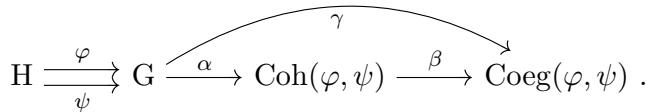
\includegraphics[keepaspectratio]{images/part002_030b7800.jpg}}

Throughout the rest of this section, \(n^{o}\), we assume that the frame of the pair \((\varphi,\psi)\) is a connected quiver and fix a vertex \(a_{0}\) of G. Consequently, the groupoids \(\mathrm{Coh}(\varphi,\psi)\) and \(\mathrm{Coeg}(\varphi,\psi)\) are transitive.

Denote by \(\Gamma\) the quiver \((\mathrm{Som}(\mathrm{G}), \mathrm{Som}(\mathrm{H}), \mathrm{Som}(\varphi), \mathrm{Som}(\psi))\) , \(\widetilde{\Gamma}\) the graph associated with \(\Gamma\), and let \(\Omega(\widetilde{\Gamma})\) be the set of finite sequences \((z_1, \ldots, z_n)\) of arrows of \(\widetilde{\Gamma}\) , with \(n \geqslant 1\) , such that the term of \(z_i\) is the origin of \(z_{i+1}\) if \(1 \leqslant i < n\) and that the term of \(z_n\) is the origin of \(z_1\) . In No. 1 we constructed a map \(\mathbf{z} \mapsto c(\mathbf{z})\) from the set \(\Omega(\widetilde{\Gamma})\) into the set of conjugacy classes of the group \(\mathrm{Coh}(\varphi, \psi)_{a_0}\) .

Denote by \(H \times_{G} H\) the equalizer in \(H \times H\) of the quiver morphisms \(\psi \circ pr_{1}\) and \(\varphi \circ pr_{2}\) . The set of its vertices is the set of pairs \((a, b)\) of vertices of H such that \(\psi(a) = \varphi(b)\) ; the set of its arrows is the set of pairs \((f, g)\) of arrows of H such that \(\psi(f) = \varphi(g)\) ; the origin of an arrow \((f, g)\) is the vertex \((o(f), o(g))\) and its endpoint is the vertex \((t(f), t(g))\) (cf. II, p. 153).

Finally, denote by \(\mathrm{Ker}(\varphi, \psi)\) the equalizer of \(\varphi\) and \(\psi\) ; recall (II, p. 165, example 2) that this is the subquiver of H whose vertices \(a\) are those such that \(\varphi(a) = \psi(a)\) and whose arrows are the \(f \in \mathrm{Fl}(\mathrm{H})\) such that \(\varphi(f) = \psi(f)\) .

PROPOSITION 4. --- Let \(\mu\colon\mathrm{H}\times_{\mathrm{G}}\mathrm{H}\to\mathrm{H}\) be a quiver morphism such that \(\varphi\circ\mu=\varphi\circ\mathrm{pr}_{1}\) and \(\psi\circ\mu=\psi\circ\mathrm{pr}_{2}\) . Suppose that, for every pair \((a,b)\) of vertices of H such that \(\varphi(a)=\varphi(b)\) , there exists a vertex \(c\) of H such that \(\varphi(c)=\psi(b)\) and \(a=\mu(b,c)\) .

  Let \(A_{1}\) be a set of vertices of \(\mathrm{Ker}(\varphi,\psi)\) meeting each of its connected components, and let \(Z_{1}\) be the set of elements of \(\Omega(\widetilde{\Gamma})\) of the form \(((a,1))\) , where \(a\in A_{1}\). Let \(A_{2}\) be a set of vertices of \(H\times_{G}H\) meeting every connected component of \(H\times_{G}H\) and let \(Z_{2}\) be the set of triples of the form \(((a,1),(b,1),(\mu(a,b),-1))\) , for \((a,b)\) ranging over \(A_{2}\) .

Then, \(\Omega(\widetilde{\Gamma})\) is the smallest distinguished subset of \(\Omega(\widetilde{\Gamma})\) which contains \(Z_1 \cup Z_2\). In particular, the conjugacy classes \(c(\mathbf{z})\) in \(\mathrm{Coh}(\varphi, \psi)_{a_0}\) , where \(\mathbf{z}\) runs through \(Z_1 \cup Z_2\) , generate the kernel of the canonical homomorphism \(\beta_{a_0}\) of \(\mathrm{Coh}(\varphi, \psi)_{a_0}\) to \(\mathrm{Coeg}(\varphi, \psi)_{\beta(a_0)}\) .

Denote by \(Z_{1}^{\prime}\) , \(Z_{2}^{\prime}\) and \(Z^{\prime}\) the smallest distinguished subsets of \(\Omega(\widetilde{\Gamma})\) respectively containing \(Z_{1}\) , \(Z_{2}\) and \(Z_{1} \cup Z_{2}\) (II, p. 197, def. 1). The aim is to prove that \(Z^{\prime}\) is equal to \(\Omega(\widetilde{\Gamma})\). By II, p. 199, corollary 1 of prop. 1 of II, p. 197, the last assertion of the proposition will follow from this.

Lemma 1. --- a) For every vertex \(a\) of \(\operatorname{Ker}(\varphi, \psi)\) , \(((a, 1))\) belongs to \(Z_1'\) .

\begin{enumerate}
\def\labelenumi{\alph{enumi})}
\setcounter{enumi}{1}
\item
  For every vertex \((a,b)\) of \(\mathrm{H}\times_{\mathrm{G}}\mathrm{H}\) , \(((a,1),(b,1),(\mu(a,b),-1))\) belongs to \(\mathbf{Z}_2^{\prime}\) .
\item
  Let \(A_{1}^{\prime}\) be the set of vertices \(a\) of \(\operatorname{Ker}(\varphi,\psi)\) such that \(((a,1))\) belongs to \(Z_{1}^{\prime}\) . We have \(A_{1}\subset A_{1}^{\prime}\) , by definition of \(Z_{1}^{\prime}\) . Let \(f\) be an arrow of \(\operatorname{Ker}(\varphi,\psi)\) , let \(a\) be its source and \(b\) its target. It follows from property (iv) in the definition of a distinguished subset (II, p. 197, def. 1) applied to the sequence \(((f,1))\) that \(a\in A_{1}^{\prime}\) is equivalent to \(b\in A_{1}^{\prime}\) . Since \(A_{1}\) meets every connected component of \(\operatorname{Ker}(\varphi,\psi)\) , we have \(A_{1}^{\prime}=\operatorname{Som}(\operatorname{Ker}(\varphi,\psi))\) , which is what had to be proved.
\item
  Let \(A_{2}^{\prime}\) be the set of vertices \((a,b)\) of \(H \times_{G} H\) such that the triple \(((a,1),(b,1),(\mu(a,b),-1))\) belongs to \(Z_{2}^{\prime}\) . By hypothesis, one has \(A_{2} \subset A_{2}^{\prime}\) . Since \(A_{2}\) meets each connected component of \(H \times_{G} H\) , it suffices to establish that, if there exists an arrow \((f,f^{\prime})\) joining a vertex \((a', b')\) to a vertex \((a, b)\) , then \((a, b)\) belongs to \(A_2'\) if and only if the same is true of \((a', b')\) .
\end{enumerate}

Let us set \(f'' = \mu(f, f')\) ; it is an arrow joining \(\mu(a', b')\) to \(\mu(a, b)\) and one has \(\varphi(f'') = \varphi(f)\) and \(\psi(f'') = \psi(f')\) . By condition (iv) in the definition of a distinguished subset of \(\Omega(\widetilde{\Gamma})\) (loc. cit.) applied to the sequence \(((f, 1), (f', 1), (f'', -1))\) , the two conditions

\begin{enumerate}
\def\labelenumi{(\roman{enumi})}
\item
  the triple \(((a,1),(b,1),(\mu (a,b), - 1))\) belongs to \(Z^{\prime}\) ;
\item
  the triple \(((a',1),(b',1),(\mu(a',b'),-1))\) belongs to \(Z'\) are equivalent. This shows that \((a,b)\) belongs to \(A_{2}'\) if and only if \((a',b')\) belongs to \(A_{2}'\) and concludes the proof of the lemma.
\end{enumerate}

We now prove by induction on the integer \(n \geqslant 1\) that every element \(((a_1, \varepsilon_1), (a_2, \varepsilon_2), \ldots, (a_n, \varepsilon_n))\) of \(\Omega(\widetilde{\Gamma})\) belongs to \(Z'\) .

\casehead{Case where \(n = 1\)}

Let \(((a,\varepsilon))\) be an element of \(\Omega(\tilde{\Gamma})\) of length 1. We have \(\varphi(a)=\psi(a)\) , whence \(((a,1))\in\mathbb{Z}'\). By Lemma 1, condition (ii) in the definition of a distinguished subset then implies that \(((a,-1))\) belongs to \(Z'\) .

\casehead{Case where \(n \geqslant 2\)}

By virtue of condition (ii) of a distinguished subset, it suffices to treat the case where \(\varepsilon_{2}=1\). Suppose that \(\varepsilon_{1}=1\) ; then, \((a_{1},a_{2})\) is a vertex of H \(\times_{G}H\) ; set \(a=\mu(a_{1},a_{2})\) ; by Lemma 1, the triple \(((a_{1},1),(a_{2},1),(a,-1))\) therefore belongs to \(Z'\). In the case where \(\varepsilon_{1}=-1\) , we have \(\varphi(a_{1})=\varphi(a_{2})\) ; one can therefore choose a vertex \(a\) of H such that \(\mu(a_{2},a)=a_{1}\) and the triple \(((a_{2},1),(a,1),(a_{1},-1))\) belongs to \(Z'\) , so the triple \(((a_{1},-1),(a_{2},1),(a,1))\) also belongs to \(Z'\), by virtue of condition (ii) in the definition of a distinguished subset.

Then, \(((a,\varepsilon_1),(a_3,\varepsilon_3),\ldots ,(a_n,\varepsilon_n))\) belongs to \(\Omega (\widetilde{\Gamma})\) and is of length \(n - 1\). By induction, this is an element of \(\mathbf{Z}'\) . Using conditions (i), (ii), and (iii) of the definition of a distinguished subset, we successively deduce that the elements

\[
\begin{array}{c} ((a _ {1}, \varepsilon_ {1}), (a _ {2}, 1), (a, - \varepsilon_ {1}), (a, \varepsilon_ {1}), (a _ {3}, \varepsilon_ {3}), \ldots , (a _ {n}, \varepsilon_ {n})), \\ ((a, - \varepsilon_ {1}), (a, \varepsilon_ {1}), (a _ {3}, \varepsilon_ {3}), \ldots , (a _ {n}, \varepsilon_ {n}), (a _ {1}, \varepsilon_ {1}), (a _ {2}, 1)), \\ ((a _ {3}, \varepsilon_ {3}), \ldots , (a _ {n}, \varepsilon_ {n}), (a _ {1}, \varepsilon_ {1}), (a _ {2}, 1)), \\ ((a _ {1}, \varepsilon_ {1}), (a _ {2}, 1), (a _ {3}, \varepsilon_ {3}), \ldots , (a _ {n}, \varepsilon_ {n})) \end{array}
\]

belong to Z'. This completes the proof of the proposition.

COROLLARY. --- a) With the notations of Proposition 4, suppose further that the map (Som(φ), Som(ψ)) from Som(H) into Som(G) × Som(G) is injective and that its image is the graph of an equivalence relation on Som(G). Then, for every vertex (a, b) of H \(\times_{G}\) H, there exists a unique vertex \(c_{a,b}\) of H such that \(\varphi(c_{a,b}) = \varphi(a)\) and \(\psi(c_{a,b}) = \psi(b)\) .

\begin{enumerate}
\def\labelenumi{\alph{enumi})}
\setcounter{enumi}{1}
\tightlist
\item
  Suppose further that for every arrow \((f, f')\) of H \(\times_{G}\) H, there exists an arrow \(f''\) of H such that \(\varphi(f'') = \varphi(f)\) and \(\psi(f'') = \psi(f')\) .
\end{enumerate}

Let A be a set of vertices of H \(\times_{G}\) H meeting each of its connected components. Then, the kernel of the morphism \(\beta_{a_{0}}\) is the smallest normal subgroup of \(\mathrm{Coh}(\varphi,\psi)_{a_{0}}\) which contains the conjugacy classes \(c((a,1),(b,1),(c_{a,b},-1))\) , for \((a,b)\in\mathrm{A}\) .

Let R be the equivalence relation on \(\operatorname{Som}(\mathrm{G})\) whose graph is the image of the mapping \((\operatorname{Som}(\varphi),\operatorname{Som}(\psi))\) . Let \((a,b)\) be a vertex of \(H\times_{G}H\) . One thus has \(\operatorname{R}\{\varphi(a),\psi(a)\}\) and \(\operatorname{R}\{\varphi(b),\psi(b)\}\) , whence \(\operatorname{R}\{\varphi(a),\psi(b)\}\) since \(\psi(a)=\varphi(b)\) . Hence, there exists a unique vertex \(c\) of H such that \(\varphi(c)=\varphi(a)\) and \(\psi(c)=\psi(b)\) ; it is denoted \(\mu(a,b)\) .

For every arrow \((f, f')\) of \(H\times_{G}H\), choose an arrow \(f''\) of H such that \(\varphi(f'') = \varphi(f)\) and \(\psi(f'') = \psi(f')\) and denote it \(\mu(f, f')\) .

We have thus defined a quiver morphism \(\mu\colon\mathrm{H}\times_{\mathrm{G}}\mathrm{H}\to\mathrm{H}\) such that \(\varphi\circ\mu=\varphi\circ\mathrm{pr}_{1}\) and \(\psi\circ\mu=\psi\circ\mathrm{pr}_{2}\) .

Let \((a,b)\) be a pair of vertices of H such that \(\varphi(a)=\varphi(b)\) . We have \(\mathrm{R}\{\varphi(a),\psi(a)\}\) and \(\mathrm{R}\{\varphi(b),\psi(b)\}\) , therefore \(\mathrm{R}\{\psi(b),\psi(a)\}\) . There consequently exists a unique vertex \(c\) of H such that \(\varphi(c)=\psi(b)\) and \(\psi(c)=\psi(a)\) . The vertex \(\mu(b,c)\) satisfies \(\varphi(\mu(b,c))=\varphi(b)=\varphi(a)\) and \(\psi(\mu(b,c))=\psi(c)=\psi(a)\) . We therefore have \(\mu(b,c)=a\) since the map \((\operatorname{Som}(\varphi),\operatorname{Som}(\psi))\) of \(\operatorname{Som}(\operatorname{H})\) into \(\operatorname{Som}(\operatorname{G})\times\operatorname{Som}(\operatorname{G})\) is injective.

Let \(A_{1}\) be the set of vertices of \(\operatorname{Ker}(\varphi,\psi)\) and let \(Z_{1}\) be the set of elements of \(\Omega(\widetilde{\Gamma})\) of the form \(((a,1))\) , for \(a\in A_{1}\) . Set \(A_{2}=A\) and let \(Z_{2}\) be the set of elements \(((a,1),(b,1),(\mu(a,b),-1))\) of \(\Omega(\widetilde{\Gamma})\) , for \((a,b)\in A_{2}\) . Denote by \(\widetilde{Z}\) (resp. \(\widetilde{Z}_{1}\), respectively \(\widetilde{Z}_{2}\)) the smallest distinguished subset of \(\Omega(\widetilde{\Gamma})\) containing \(Z_{1}\cup Z_{2}\) (resp. \(Z_{1}\), respectively \(Z_{2}\)).

Let \(a \in \mathrm{A}_1\). We have \(\varphi(a) = \psi(a)\) ; set \(x = \varphi(a)\). The vertex \(a\) is the unique vertex of H such that \(\varphi(a) = \psi(a) = x\). In particular, we have \(\mu(a, a) = a\). The triple \(((a, 1), (a, 1), (a, -1))\) therefore belongs to \(\mathbf{Z}_2\). It then follows from conditions (i) and (iii) in the definition of a distinguished subset that \(((a, 1))\) belongs to \(\widetilde{\mathbf{Z}}_2\). Consequently, we have \(\mathbf{Z}_1 \subset \widetilde{\mathbf{Z}}_2\) , whence \(\widetilde{\mathbf{Z}} = \widetilde{\mathbf{Z}}_2\) .

By Proposition 4, \(\Omega(\tilde{\Gamma})\) is the smallest distinguished subset of \(\Omega(\tilde{\Gamma})\) containing \(Z_{2}\), and the kernel of \(\beta_{a_{0}}\) is the smallest normal subgroup of \(\mathrm{Coh}(\varphi,\psi)_{a_{0}}\) which contains the conjugacy classes \(c(\mathbf{z})\) , for \(\mathbf{z}\in Z_{2}\) . Hence the corollary.

Example. --- Let X and R be topological spaces, let o and t be continuous maps from R to X, and let C be the set of pairs \((f,g)\in\mathrm{R}^{2}\) such that \(t(f)=o(g)\) in R and let m be a continuous map from C to R that makes the quiver \((\mathrm{X},\mathrm{R},o,t)\) a groupoid; suppose further that the map \(f\mapsto f^{-1}\) from R to R is continuous. The hypotheses of the proposition are then satisfied if one sets \(\mathrm{H}=\varpi(\mathrm{R})\) , \(\mathrm{G}=\varpi(\mathrm{X})\) , \(\varphi=\varpi(o)\) , \(\psi=\varpi(t)\) and \(\mu=\varpi(m)\) .

Suppose further that R is the graph of an equivalence relation on X, with the maps o and t being derived from the projections of \(X \times X\) in X by passing to subspaces. The hypotheses of the corollary are then satisfied.

Remark. --- *More generally, the hypotheses of the proposition are satisfied when (G, H, \(\varphi\) , \(\psi\) , \(\mu\) ) is a “groupoid of groupoids.” This means that G and H are groupoids, \(\varphi\) and \(\psi\) are morphisms of groupoids from H to G, making the quadruple (G, H, \(\varphi\) , \(\psi\) ) a “groupoid quiver”; finally, \(\mu\) is a composition law in this “quiver” given by a groupoid morphism H \(\times_{\mathrm{G}}\) H → H, satisfying a certain number of properties expressing the associativity of the law and the fact that every “arrow” is invertible. The reader will also note that the applications to the fundamental groupoid studied in this work all fall within this case.

\subsection{Isotropy group of a coequalizer}

Let G and H be groupoids; let \(\varphi\) and \(\psi\) morphisms of groupoids from H to G. The purpose of this section is to summarize the computation of the isotropy groups of the cohomotoper (II, p. 193, prop. 6) and the comparison of the isotropy groups of the cohomotoper and of the coequalizer made in the preceding section, in order to deduce from this the computation of the isotropy groups of the coequalizer Coeg( \(\varphi\) , \(\psi\) ).

Denote by \(\alpha\colon\mathrm{G}\to\mathrm{Coh}(\varphi,\psi)\) , \(\beta\colon\mathrm{Coh}(\varphi,\psi)\to\mathrm{Coeg}(\varphi,\psi)\) and \(\gamma=\beta\circ\alpha\colon\mathrm{G}\to\mathrm{Coeg}(\varphi,\psi)\) the canonical groupoid morphisms. Denote \(h\colon\mathrm{Som}(\mathrm{H})\to\mathrm{Fl}(\mathrm{Coh}(\varphi,\psi))\) the canonical homotopy; recall that the set of vertices of \(\mathrm{Coh}(\varphi,\psi)\) is equal to \(\mathrm{Som}(\mathrm{G})\) .

Denote by \(\Gamma\) the quiver (Som(G), Som(H), Som(φ), Som(ψ)), denote then \(\varphi_0\) and \(\psi_0\) the maps induced by \(\varphi\) and \(\psi\) by passing to orbits and \(\Gamma_0\) the frame (Orb(G), Orb(H), \(\varphi_0, \psi_0\) ) of the pair ( \(\varphi, \psi\) ). We shall assume that the quiver \(\Gamma_0\) is connected and its vertex set is nonempty, which amounts to assuming that the groupoids Coh(φ, ψ) and Coeg(φ, ψ) are transitive.

Recall (cf. II, p. 192, definition 4) that a base equipment consists of the data of a family \((a, b, c_1, c_2, \mathrm{T}, i_0)\) where: for all \(i \in \mathrm{Orb}(\mathrm{G})\) , \(a(i)\) is a vertex in the orbit \(i\) of \(\mathrm{G}\) ; for every \(j \in \mathrm{Orb}(\mathrm{H})\) , \(b(j)\) is a vertex in the orbit \(j\) of \(\mathrm{H}\) , \(c_1(j)\) and \(c_2(j)\) are arrows from \(\mathrm{G}\) respectively \(\varphi(b(j))\) to \(a(\varphi_0(j))\) and \(\psi(b(j))\) to \(a(\psi_0(j))\) ; \(\mathrm{T}\) is a subquiver of \(\Gamma_0\) whose associated tree is a maximal tree of the graph \(\widetilde{\Gamma}_0\) ; finally, \(i_0\) is an orbit of \(\mathrm{G}\) and we set \(a_0 = a(i_0)\) .

We then define a quiver morphism \(\tau_0\) from \(\Gamma_0\) to \(\mathrm{Coh}(\varphi, \psi)\) such that \(\tau_0(i) = \beta(a(i))\) and \(\tau_0(j) = \alpha(c_1(j))^{-1}h(b(j))\alpha(c_2(j))\) for \(i \in \mathrm{Orb}(\mathrm{G})\) and \(j \in \mathrm{Orb}(\mathrm{H})\) . If \(i\) belongs to \(\mathrm{Orb}(\mathrm{G})\) , let \(d_i\) be the unique class of paths in the graph \(\widetilde{\mathrm{T}}\) connecting \(i_0\) to \(i\) and denote by \(\delta_i\) its image in \(\mathrm{Coh}(\varphi, \psi)\) by the groupoid morphism \(\tau_0\) .

From these data, prop. 6 (II, p. 193) yields a surjective homomorphism.

\[
\Lambda \colon \bigl (\underset {i \in \pi_ {0} (\mathrm{G})} {*} \mathrm{G} _ {a (i)} \bigr) * \mathrm{F} (\operatorname{Orb} (\mathrm{H})) \to \operatorname{Coh} (\varphi , \psi) _ {a (i _ {0})}
\]

and describes generators of its kernel, thereby providing a presentation of the group \(\mathrm{Coh}(\varphi,\psi)_{a_{0}}\) .

The set of loops of length \(\geqslant 1\) in the graph \(\widetilde{\Gamma}\) associated with \(\Gamma\) is identified with the set \(\Omega(\widetilde{\Gamma})\) of sequences \((z_1, \ldots, z_n)\) of arrows of \(\widetilde{\Gamma}\) , indexed by \(\mathbf{Z}/n\mathbf{Z}\) , where \(n\) runs through the set of integers \(\geqslant 1\) , such that for every \(k \in \mathbf{Z}/n\mathbf{Z}\) , the term of \(z_k\) is the origin of \(z_{k+1}\) . Let \(\mathbf{Z}\) be a subset of \(\Omega(\widetilde{\Gamma})\) such that the conjugacy classes \(c(z)\) , for \(z \in \mathbf{Z}\) , generate the kernel of the surjective homomorphism \(\beta_{a_0}\) . The homomorphism \(\beta_{a_0} \circ \Lambda\) is surjective; to deduce its kernel from this, that is, a presentation of the group \(\operatorname{Coeg}(\varphi, \psi)_{\beta(a_0)}\) , it remains to choose, for every \(z \in \mathbf{Z}\) , an element \(\mathrm{C}(z)\) in the group \(\left( \begin{array}{cc} * & \mathrm{G}_{a(i)} \\ i \in \mathrm{Orb}(\mathrm{G}) & \end{array} \right) * \mathrm{F}(\pi_0(\mathrm{H}))\) such that \(\Lambda(\mathrm{C}(z))\) belongs to the conjugacy class \(c(z)\) .

So let \(z = (z_{1}, \ldots, z_{n})\) be an element of \(\Omega(\tilde{\Gamma})\) ; set \(z_{k} = (y_{k}, \varepsilon_{k})\) , where \(y_{k} \in \mathrm{Fl}(\Gamma) = \mathrm{Som}(\mathrm{H})\) and \(\varepsilon_{k} \in \{\pm 1\}\) . By definition, \(c(z)\) is the conjugacy class of the element

\[
g h (y _ {1}) ^ {\varepsilon_ {1}} \dots h (y _ {n}) ^ {\varepsilon_ {n}} g ^ {- 1}
\]

of the group \(\mathrm{Coh}(\varphi,\psi)_{a_{0}}\) , where g is an arbitrary arrow in \(\mathrm{Coh}(\varphi,\psi)\) connecting \(a_{0}\) to the origin of \(z_{1}\) . For \(k \in Z/nZ\) , let \(j_{k}\) be the orbit of \(y_{k}\) in H and choose an arrow \(f_{k}\) of H connecting \(y_{k}\) to the vertex \(b(j_{k})\). By definition of a homotopy, we then have the relation

\[
h (y _ {k}) (\alpha \circ \psi) (f _ {k}) = (\alpha \circ \varphi) (f _ {k}) h (b (j _ {k}))
\]

in the groupoid \(\mathrm{Coh}(\varphi,\psi)\) . Consequently, using the definition of the quiver morphism \(\tau_{0}\) , we have

\[
\begin{array}{l} h (y _ {k}) = (\alpha \circ \varphi) (f _ {k}) \cdot h (b (j _ {k})) \cdot (\alpha \circ \psi) (f _ {k}) ^ {- 1} \\ \quad = (\alpha \circ \varphi) (f _ {k}) \cdot (\alpha \circ c _ {1}) (j _ {k}) \cdot \tau_ {0} (j _ {k}) \cdot (\alpha \circ c _ {2}) (j _ {k}) ^ {- 1} \cdot (\alpha \circ \psi) (f _ {k}) ^ {- 1} \\ \quad = (\alpha \circ \varphi) (f _ {k}) \cdot (\alpha \circ c _ {1}) (j _ {k}) \cdot \delta_ {\varphi_ {0} (j _ {k})} ^ {- 1} \cdot \\ \quad \cdot \delta_ {\varphi_ {0} (j _ {k})} \cdot \tau_ {0} (j _ {k}) \cdot \delta_ {\psi_ {0} (j _ {k})} ^ {- 1} \cdot \\ \quad \cdot \delta_ {\psi_ {0} (j _ {k})} \cdot (\alpha \circ c _ {2}) (j _ {k}) ^ {- 1} \cdot (\alpha \circ \psi) (f _ {k}) ^ {- 1} \\ = u _ {k} \Lambda (j _ {k}) v _ {k}, \end{array}
\]

where we have set

\[
u _ {k} = \alpha (\varphi (f _ {k}) c _ {1} (j _ {k})) \cdot \delta_ {\varphi_ {0} (j _ {k})} ^ {- 1} \quad \text { and } \quad v _ {k} = \delta_ {\psi_ {0} (j _ {k})} \cdot \alpha (\psi (f _ {k}) c _ {2} (j _ {k})) ^ {- 1}.
\]

For every element \(k \in \mathbf{Z}/n\mathbf{Z}\) , define arrows \(\widetilde{u}_{k}, \widetilde{v}_{k}\) in G by

\[
h (y _ {k}) ^ {\varepsilon_ {k}} = \widetilde {u} _ {k} \Lambda (j _ {k}) ^ {\varepsilon_ {k}} \widetilde {v} _ {k},
\]

so that

\[
(\widetilde {u} _ {k}, \widetilde {v} _ {k}) = \left\{ \begin{array}{l l} (u _ {k}, v _ {k}) & \text { if } \varepsilon_ {k} = 1; \\ (v _ {k} ^ {- 1}, u _ {k} ^ {- 1}) & \text { if } \varepsilon_ {k} = - 1. \end{array} \right.
\]

Denote by \(x_{k}\) the origin of the arrow \(h(y_{k})^{\varepsilon_{k}}\) ; its target is then \(x_{k+1}\) ; let \(i_{k}\) be the orbit of \(x_{k}\) . Let us then define a loop \(\lambda_{k}(z)\) at \(a(i_{k})\) in the groupoid G by the formula

\[
\lambda_ {k} (z) = \left\{ \begin{array}{l l} c _ {2} (j _ {k - 1}) ^ {- 1} \psi (f _ {k - 1}) ^ {- 1} \varphi (f _ {k}) c _ {1} (j _ {k}) & \text {if} (\varepsilon_ {k - 1}, \varepsilon_ {k}) = (1, 1); \\ c _ {2} (j _ {k - 1}) ^ {- 1} \psi (f _ {k - 1}) ^ {- 1} \psi (f _ {k}) c _ {2} (j _ {k}) & \text {if} (\varepsilon_ {k - 1}, \varepsilon_ {k}) = (1, - 1); \\ c _ {1} (j _ {k - 1}) ^ {- 1} \varphi (f _ {k - 1}) ^ {- 1} \varphi (f _ {k}) c _ {1} (j _ {k}) & \text {if} (\varepsilon_ {k - 1}, \varepsilon_ {k}) = (- 1, 1); \\ c _ {1} (j _ {k - 1}) ^ {- 1} \varphi (f _ {k - 1}) ^ {- 1} \psi (f _ {k}) c _ {2} (j _ {k}) & \text {if} (\varepsilon_ {k - 1}, \varepsilon_ {k}) = (- 1, - 1) \end{array} \right.\tag{1}
\]

By construction, we have

\[
\Lambda (\lambda_ {k} (z)) = \widetilde {v} _ {k - 1} \widetilde {u} _ {k},
\]

so that the image under the homomorphism \(\Lambda\) of the element

\[
\mathrm{C} (z) = \lambda_ {1} (z) (j _ {1}) ^ {\varepsilon_ {1}} \lambda_ {2} (z) (j _ {2}) ^ {\varepsilon_ {2}} \dots \lambda_ {n} (z) (j _ {n}) ^ {\varepsilon_ {n}}\tag{2}
\]

belongs to the conjugacy class \(c(z)\) .

DEFINITION 3. --- Let G and H be groupoids; let \(\varphi\) and \(\psi\) morphisms of groupoids from H to G. We assume that the groupoid Coeg \((\varphi, \psi)\) is transitive. Let \((a, b, c_1, c_2, T, i_0)\) be a basic equipment of the pair \((\varphi, \psi)\) .

One calls complementary equipment the data of a subset Z of \(\Omega(\widetilde{\Gamma})\) such that the conjugacy classes \(c(\mathbf{z})\) for \(\mathbf{z} \in \mathbf{Z}\) generate the kernel of the homomorphism \(\beta_{a(i_0)}\) and, for every element \(\mathbf{z} = ((y_1, \varepsilon_1), \ldots, (y_n, \varepsilon_n))\) of Z, a sequence \(f(\mathbf{z}) = (f_1, \ldots, f_n)\) of arrows in H such that \(f_k\) connects \(y_k\) to the vertex \(b(j_k)\) , \(j_k\) denoting the orbit of \(y_k\) in H.

A complete equipment of the pair \((\varphi,\psi)\) is the data of a base equipment and a complementary equipment.

PROPOSITION 5. --- Let G and H be groupoids; let \(\varphi\) and \(\psi\) be morphisms of groupoids from H to G. Suppose that the groupoid \(\operatorname{Coeg}(\varphi, \psi)\) is transitive. Denote by \(\gamma\colon \mathrm{G} \to \mathrm{Coeg}(\varphi, \psi)\) the canonical groupoid morphism.

We equip the pair \((\varphi, \psi)\) with a complete equipment

\[
(a, b, c _ {1}, c _ {2}, \mathrm{T}, i _ {0}, \mathrm{Z}, (f (\mathbf {z})) _ {\mathbf {z} \in \mathrm{Z}}).
\]

For \(j \in \text{Orb(H)}\) , let \(\varphi_j \colon \text{H}_{b(j)} \to \text{G}_{a(\varphi_0(j))}\) and \(\psi_j \colon \text{H}_{b(j)} \to \text{G}_{a(\psi_0(j))}\) be the group homomorphisms \(\text{Int}(c_1(j))^{-1} \circ \varphi_{b(j)}\) and \(\text{Int}(c_2(j))^{-1} \circ \psi_{b(j)}\) respectively, where \(\varphi_0\) and \(\psi_0\) denote the canonical maps induced by \(\varphi\) and \(\psi\) by passing to orbits. Let \(\tau\) be the morphism of the frame \(\Gamma_0\) of the pair \((\varphi, \psi)\) into \(\text{Coeg}(\varphi, \psi)\) defined by \(\text{Som}(\tau)(i) = \gamma(a(i))\) if \(i \in \text{Orb(G)}\) and such that \(\text{Fl}(\tau)(j)\) is the path \(\gamma(c_1(j))^{-1} \gamma(c_2(j))\) in \(\text{Coeg}(\varphi, \psi)\). If \(i\) is an orbit of G, let \(c_i\) be the unique class of paths in \(\widetilde{\text{T}}\) connecting \(i_0\) to \(i\), and set \(\delta_i = \widetilde{\tau}(c_i)\) , where \(\widetilde{\tau} \colon \text{Grp(G)} \to \text{Coeg}(\varphi, \psi)\) is the canonical groupoid morphism induced by \(\tau\) .

There then exists a unique group homomorphism

\[
\lambda \colon \bigl ( \begin{array}{c} * \\ i \in \operatorname{Orb} (\mathrm{G}) \end{array} \mathrm{G} _ {a (i)} \bigr) * \mathrm{F} (\operatorname{Orb} (\mathrm{H})) \to \operatorname{Coeg} (\varphi , \psi) _ {\gamma (a (i _ {0}))}
\]

such that

\[
\begin{array}{l l} \lambda (f) = \delta_ {i} \gamma_ {a (i)} (f) \delta_ {i} ^ {- 1} & \text { for } i \in \mathrm{Orb(G)} \text { and } f \in \mathrm{G} _ {a (i)}, \\ \lambda (j) = \delta_ {\varphi_ {0} (j)} \tau (j) \delta_ {\psi_ {0} (j)} ^ {- 1} & \text { for } j \in \mathrm{Orb(H)}. \end{array}
\]

The homomorphism \(\lambda\) is surjective; its kernel is the smallest normal subgroup containing the following elements:

\[
\left(\mathrm{R} _ {1}\right) \quad r _ {1} (j) = j \quad \text { for } j \text { in } \mathrm{Fl} (\mathrm{T});
\]

\[
(\mathrm{R} _ {2}) \quad r _ {2} (j, f) = \varphi_ {j} (f) j \psi_ {j} (f) ^ {- 1} j ^ {- 1}
\]

\[
\text { for } j \in \operatorname{Orb} (\mathrm{H}) \text { and } f \in \mathrm{H} _ {b (j)};\tag{\((R_{3})\)}
\]

\[
r _ {3} (z) = \lambda_ {1} (z) j _ {1} ^ {\varepsilon_ {1}} \lambda_ {2} (z) j _ {2} ^ {\varepsilon_ {2}} \dots \lambda_ {n} (z) j _ {n} ^ {\varepsilon_ {n}}
\]

\[
\text { for } z = ((y _ {1}, \varepsilon_ {1}), \dots , (y _ {n}, \varepsilon_ {n})) \in \mathbf {Z},
\]

where the loops \(\lambda_{i}(z)\) are defined by formula (1), p. 208.

The existence and uniqueness of such a morphism follows from the universal property of the free product of a family of groups (A, I, p. 85, prop. 8). Denote by \(\alpha\colon G\to\mathrm{Coh}(\varphi,\psi)\) and \(\beta\colon\mathrm{Coh}(\varphi,\psi)\to\mathrm{Coeg}(\varphi,\psi)\) the canonical morphisms, so that \(\gamma=\beta\circ\alpha\). Let also \(h\colon\mathrm{Som}(H)\to\mathrm{Fl}(\mathrm{Coh}(\varphi,\psi))\) be the canonical homotopy relating \(\alpha\circ\varphi\) to \(\alpha\circ\psi\) . Since \(\beta\) is the groupoid morphism obtained by contracting the arrows of the image of \(h\) , we have

\[
\operatorname{Fl} (\tau) (j) = \gamma (c _ {1} (j)) ^ {- 1} \gamma (c _ {2} (j)) = \gamma (c _ {1} (j) ^ {- 1}) \beta (h (j)) \gamma (c _ {2} (j)) = \beta (\tau_ {0} (j))
\]

in \(\operatorname{Coeg}(\varphi,\psi)\) , where \(\tau_{0}\colon\Gamma_{0}\to\mathrm{Coh}(\varphi,\psi)\) denotes the quiver morphism induced by the base equipment \((a,b,c_{1},c_{2},\mathrm{T},i_{0})\) . Consequently, the homomorphism \(\lambda\) is the composite of the homomorphism \(\Lambda\) defined in Prop. 6 (II, p. 193) and of the surjective homomorphism \(\beta_{a(i_0)}\) . It is in particular surjective.

Let \(z \in \mathbf{Z}\). By construction, \(\Lambda(r_3(z))\) belongs to the conjugacy class \(c(z)\) . By definition of a complementary equipment, the kernel of the homomorphism \(\beta_{a(i_0)}\) is therefore the smallest normal subgroup of \(\mathrm{Coh}(\varphi, \psi)_{a(i_0)}\) containing the elements \(\Lambda(r_3(z))\) for \(z \in \mathbf{Z}\) . Since the homomorphism \(\Lambda\) is surjective, the kernel of the homomorphism \(\lambda = \beta_{a(i_0)} \circ \Lambda\) is therefore the smallest normal subgroup of the group \(\left( *_{i \in \mathrm{Orb}(G)} G_{a(i)} \right) * F(\pi_0(H))\) containing the generators of the kernel of \(\Lambda\) given by the formulas \((R_1), (R_2)\) , as well as the elements defined by the formulas \((R_3)\) . The proposition is thus proved.

\subsection{Quotient of a groupoid by the action of a group}

Let G be a transitive groupoid, let K be a group, and let \(\theta\colon\mathrm{K}\to\mathrm{Aut}(\mathrm{G})^{\circ}\) be a group homomorphism from K into the opposite group of the automorphism group of the groupoid G. We will say that the group K acts on the right on G. If \(k\in\mathrm{K}\) we will sometimes denote by \(k^{*}x\) (resp. \(k^{*}f\) ) the image of a vertex \(x\) (resp. of an arrow \(f\) ) of G under the groupoid automorphism \(\theta(k)\) .

Let \(|\mathrm{K}|\) be the groupoid whose set of vertices is \(\mathrm{K}\) and whose set of arrows connecting two vertices is empty if these vertices are distinct, and is reduced to a single element otherwise. Let \(\mathrm{H}\) be the product groupoid \(\mathrm{G} \times |\mathrm{K}|\) ; a vertex of \(\mathrm{H}\) is a pair \((a,k)\) , where \(a\) is a vertex of \(\mathrm{G}\) and \(k\) is an element of \(\mathrm{K}\) ; if \(f\) is an arrow of \(\mathrm{G}\) joining a vertex \(a\) to a vertex \(b\) , we shall denote \((f,k)\) the unique arrow of \(\mathrm{H}\) connecting \((a,k)\) to \((b,k)\) . Let \(\varphi: \mathrm{H} \to \mathrm{G}\) be the groupoid morphism given by the first projection, and let \(\psi: \mathrm{H} \to \mathrm{G}\) be the groupoid morphism such that \(\operatorname{Som}(\psi)((a,k)) = k^*a\) and \(\operatorname{Fl}(\psi)((f,k)) = k^*f\) if \(k \in \mathrm{K}\) , \(a \in \operatorname{Som}(\mathrm{G})\) and \(f \in \operatorname{Fl}(\mathrm{G})\) .

Let G/K denote the coequalizer \(\operatorname{Coeg}(\varphi,\psi)\) and let \(\gamma\colon G\to G/K\) be the canonical groupoid morphism.

Let o be a vertex of G. For \(k \in K\), choose an arrow \(c_{k}\) connecting \(k^{*}o\) to o in G; such an arrow exists because G is transitive. For \(k \in K\), denote by \(\text{Fix}(k)\) the subgroupoid of G whose vertices (resp. arrows) are the elements of \(\text{Som}(G)\) (resp. of \(\text{Fl}(G)\) ) fixed by k; let us choose a set \(A_{k}\) of vertices of \(\text{Fix}(k)\) meeting all the orbits of this groupoid. For \(k \in K\) and \(a \in A_{k}\) we also choose an arrow \(f_{(a,k)}\) in G connecting the vertex a to the vertex o.

Proposition 6. — The unique group homomorphism

\[
\lambda \colon \mathrm{G} _ {o} * \mathrm{F} (\mathrm{K}) \to (\mathrm{G} / \mathrm{K}) _ {\gamma (o)}
\]

such that \(\lambda(f) = \gamma_o(f)\) for \(f \in \mathrm{G}_o\) and \(\lambda([k]) = \gamma(c_k)\) for \(k \in \mathrm{K}\) is surjective. Its kernel is the smallest normal subgroup of \(\mathrm{G}_o * \mathrm{F}(\mathrm{K})\) containing the following elements:

\[
r _ {2} (k, f) = [ k ] ^ {- 1} f [ k ] (c _ {k} ^ {- 1} k ^ {*} (f) ^ {- 1} c _ {k})\tag{\((R_{2})\)}
\]

\[
\text { for } k \in \mathrm{K} \text { and } f \in \mathrm{G} _ {o};\tag{\((\mathrm{R}_{3}^{\prime})\)}
\]

\[
r _ {3} ^ {\prime} (k, a) = [ k ] (c _ {k} ^ {- 1} k ^ {*} (f _ {(a, k)}) ^ {- 1} f _ {(a, k)}))
\]

\[
\text { for } k \in \mathrm{K} - \{e \} \text { and } a \in \mathrm{A} _{k}\tag{\((\mathrm{R}_{3}^{\prime\prime})\)}
\]

\[
r _ {3} ^ {\prime \prime} (k, h) = [ k h ] ^ {- 1} [ k ] [ h ] (c _ {h} ^ {- 1} h ^ {*} (c _ {k} ^ {- 1}) c _ {k h})
\]

\[
\text { for } k,h \in \mathrm{K}.
\]

Since G is transitive, the map which associates to an element \(k \in K\) the orbit of \((o, k)\) is a bijection from K onto the set of orbits of H. We thus identify \(\operatorname{Orb}(\mathbf{G})\) with \(\{o\}\) and \(\operatorname{Orb}(\mathbf{H})\) with K. The frame \(\Gamma_{0}\) of the pair \((\varphi, \psi)\) then identifies with the quiver having a single vertex o and whose set of arrows is K. Let T be the subquiver of \(\Gamma_{0}\) of vertex set \(\{o\}\) and whose set of arrows is empty; the associated graph is the unique maximal tree of the graph \(\widetilde{\Gamma}_{0}\).

The family \((o,(o,k)_{k\in \mathrm{K}},(e_o)_{k\in \mathrm{K}},(c_k)_{k\in \mathrm{K}},\mathrm{T},o)\) is a base equipment of the pair \((\varphi ,\psi)\) .

The map \(f \mapsto (f, k)\) defines an isomorphism of the isotropy group \(G_o\) onto the isotropy group \(H_{(o,k)}\) ; under this isomorphism, the homomorphisms \(\varphi_k\) and \(\psi_k\) of \(H_{(o,k)}\) into \(G_o\) defined by prop. 5 of II, p. 208 are given by

\[
\varphi_ {k} (f, k) = f \quad \text { and } \quad \psi_ {k} (f, k) = c _ {k} ^ {- 1} k ^ {*} (f) c _ {k},\tag{3}
\]

for \(k\in \mathrm{K}\) and \(f\in \mathrm{G}_o\).

The quiver \(H \times_{G} H\) is the equalizer in \(H \times H\) of quiver morphisms \(\psi \circ pr_{1}\) and \(\varphi \circ pr_{2}\) . Its vertices are the pairs \(((a, k), (b, h))\) where a and b are vertices of G and k and h are elements of K such that \(b = k^{*}a\) , and its arrows are the pairs \(((f, k), (g, h))\) where f and g are arrows of G, and k and h are elements of K such that \(g = k^{*}f\) ; the origin of the arrow \(((f,k),(g,h))\) is equal to \(((o(f),k),(o(g),h))\) ; its target is equal to \(((t(f),k),(t(g),h))\) .

We then define a quiver morphism \(\mu\) of \(H \times_{\mathrm{G}} H\) into H by setting \(\mu((a,k),(b,h)) = (a,kh)\) and \(\mu((f,k),(g,h)) = (f,kh)\) . We have \(\varphi \circ \mu = \varphi \circ \mathrm{pr}_1\) and \(\psi \circ \mu = \psi \circ \mathrm{pr}_2\) .

Let \(x\) and \(y\) be vertices of H such that \(\varphi(x) = \varphi(y)\). There thus exists a vertex \(a\) of G and elements \(k\) and \(h\) of K such that \(x = (a, k)\) and \(y = (a, h)\) . Set \(z = (h^* a, h^{-1} k)\) ; we have \(\mu(y, z) = x\). This shows that the pair \((\varphi, \psi)\) satisfies the hypotheses of Prop. 4 (II, p. 202).

A vertex \((a,k)\) of H belongs to the groupoid \(\operatorname{Ker}(\varphi,\psi)\), equalizer of \(\varphi\) and \(\psi\), if and only if \(k^{*}a=a\), that is, if k belongs to the stabilizer of the vertex a in the group K. Let \(A_{1}\) be the set of pairs \((a,k)\), for \(k\in K\) and \(a\in A_{k}\); it meets all the orbits of the subgroupoid \(\operatorname{Ker}(\varphi,\psi)\) of H. Let \(Z_{1}\) be the part of \(\Omega(\widetilde{\Gamma})\) formed of sequences of the form (((a,k),1)), for \((a,k)\in A_{1}\). For \(\mathbf{z}=((a,k),1)\in\mathbf{Z}_{1}\), \((f_{(a,k)},k)\) is an arrow of H which connects \((a,k)\) to \((o,k)\). Set \(f(\mathbf{z})=((f_{(a,k)},k))\).

The set \(\mathrm{A}_2\) of vertices of \(\mathrm{H} \times_{\mathrm{G}} \mathrm{H}\) of the form \(((o,k), (k^*o,h))\) , for \((k,h) \in \mathrm{K}^2\) , meets every orbit of \(\mathrm{H} \times_{\mathrm{G}} \mathrm{H}\) . Observe also that one has \(\mu((o,k), (k^*o,h)) = (o,kh)\) . The arrows \((e_o,k), (c_k,h), (e_o,kh)\) in H connect respectively \((o,k), (k^*o,h), (o,kh)\) to \((o,k), (o,h)\) and \((o,kh)\) . Denote by \(\mathrm{Z}_2\) the set of sequences of the form \((((o,k),1), ((k^*o,h), 1), ((o,kh), -1))\) in \(\Omega(\widetilde{\Gamma})\) ; for such an element \(\mathbf{z}\) of \(\mathrm{Z}_2\) , set \(f(\mathbf{z}) = ((e_o,k), (c_k,h), (e_o,kh))\) .

By prop. 4 of II, p. 202, the set \(Z = Z_1 \cup Z_2\) and the family \((f(\mathbf{z}))_{z \in \mathbb{Z}}\) form a complementary equipment.

Let \(k \in \mathrm{K}\) and let \(a \in \mathrm{A}_k\) . The element \(\mathrm{C}((a, k), 1)\) of the group \(\mathrm{G}_o * \mathrm{F}(\mathrm{K})\) defined by formula (2) of II, p. 208 is equal to

\[
c _ {k} ^ {- 1} \psi ((f _ {(a, k)}, k)) ^ {- 1} \varphi (f _ {(a, k)}) e _ {o} [ k ] = (c _ {k} ^ {- 1} k ^ {*} (f _ {(a, k)}) ^ {- 1} f _ {(a, k)}) [ k ].\tag{4}
\]

Let \(k,h \in \mathbf{K}\). One verifies that the element

\[
\mathrm{C} (((o, k), 1), ((k ^ {*} o, h), 1), ((o, k h), - 1))
\]

of the group \(G_{o} * F(K)\) defined by formula (2) of II, p. 208 is equal to

\[
[ k ] [ h ] (c _ {h} ^ {- 1} h ^ {*} (c _ {k} ^ {- 1}) c _ {k h}) [ k h ] ^ {- 1}.\tag{5}
\]

The elements \(r_3'(e, a)\) given by the relations \((\mathrm{R}_3')\) for \(k = e\) are all equal to \([e]c_e^{-1}\), an element of the group \(\mathrm{G}_o * \mathrm{F}(\mathrm{K})\) obtained by applying the relation \((\mathrm{R}_{3}^{\prime\prime})\) to \(k = h = e\). In view of relations (3), (4), and (5), the proposition therefore follows from II, p. 208, prop. 5.

COROLLARY 1. --- Suppose that the group K is generated by the fixators of the vertices of G. Then the group homomorphism \(\gamma_{o}\colon\mathrm{G}_{o}\to(\mathrm{G}/\mathrm{K})_{\gamma(o)}\) is surjective. Moreover, if the groupoid G is simply transitive, then so is the groupoid G/K.

The relation \((\mathrm{R}_{3}^{\prime\prime})\) implies \(\lambda([e]) = \lambda(c_{e}) = \gamma_{o}(c_{e})\) . The relations \((\mathrm{R}_{3}^{\prime\prime})\) then imply that the set of \(k \in K\) such that \(\lambda([k])\) belongs to the image of \(\gamma_{o}\) is a subgroup of K. Finally, the relations \((\mathrm{R}_{3}^{\prime})\) show that, for every element \(k \in K\) whose fixator is not empty, \(\lambda([k])\) belongs to the image of \(\gamma_{o}\) . The corollary follows from this.

Remark 1. --- One can give another description, sometimes more convenient, of the group \((\mathrm{G}/\mathrm{K})_{\gamma(o)}\). For this, set \(M = K \times G_{o}\) and let us define a composition law on M by the formula

\[
(k, a) \cdot (h, b) = (k h, c _ {k h} ^ {- 1} h ^ {*} (c _ {k} a) c _ {h} b),
\]

for \(k\) , \(h \in \mathrm{K}\) and \(a\) , \(b \in \mathrm{G}_o\) . We verify that this composition law is associative, that \((e, c_e^{-1})\) is an identity element and that the element \((k^{-1}, c_{k^{-1}}^{-1}(k^{-1})^*(c_k a)^{-1} c_e)\) is the inverse of \((k, a)\) . It therefore endows M with a group structure. Moreover, the map \(\lambda'\colon \mathrm{M} \to (\mathrm{G} / \mathrm{K})_{\gamma(o)}\) defined by \((k, a) \mapsto \lambda([k]a)\) is a group homomorphism. Let \(\alpha'\) be the unique group homomorphism from \(\mathrm{G}_o * \mathrm{F}(\mathrm{K})\) to M such that \(\alpha'(f) = (e, f)\) if \(f \in \mathrm{G}_o\) and \(\alpha'([k]) = (k, e_o)\) if \(k \in \mathrm{K}\) ; we have \(\lambda' \circ \alpha' = \lambda\) .

The relations \((\mathrm{R}_{2})\) and \((\mathrm{R}_{3}^{\prime\prime})\) show that every element of \((\mathrm{G}/\mathrm{K})_{\gamma(o)}\) is the image under the homomorphism \(\lambda\) of an element of \(\mathrm{G}_{o}*\mathrm{F}(\mathrm{K})\) of the form \([k]f\) , with \(f\in G_{o}\) and \(k\in K\) . Consequently, the homomorphism \(\lambda'\) is surjective. One also verifies that the image under \(\alpha'\) of an element of \(\mathrm{G}_{o}*\mathrm{F}(\mathrm{K})\) of the form \((\mathrm{R}_{2})\) or \((\mathrm{R}_{3}^{\prime\prime})\) is zero. Consequently, the kernel of the homomorphism \(\lambda'\) is the smallest normal subgroup of M containing the images under \(\alpha'\) of the elements of \(\mathrm{G}_{o}*\mathrm{F}(\mathrm{K})\) of the form \((\mathrm{R}_{3}^{\prime})\) .

COROLLARY 2. --- Suppose that the group K acts freely on Som(G). Then there exists a unique group homomorphism \(\pi\colon (\mathrm{G} / \mathrm{K})_{\gamma (o)}\to \mathrm{K}\) whose kernel contains the image of \(\gamma_{o}\) and such that \(\pi (\lambda ([k])) = k\) for all \(k\in \mathbf{K}\) . Moreover, \(\mathrm{G}_o\xrightarrow{\gamma_o} (\mathrm{G} / \mathrm{K})_{\gamma (o)}\xrightarrow{\pi}\mathrm{K}\) is an extension of K by \(\mathrm{G}_o\) .

If such a group homomorphism \(\pi\) exists, the group homomorphism \(\pi \circ \lambda\) is necessarily equal to the unique group homomorphism \(p\) of \(\mathrm{G}_{o} * \mathrm{F}(\mathrm{K})\) into \(\mathrm{K}\) such that \(p(f) = e\) for \(f \in \mathrm{G}_{o}\) and \(p([k]) = k\) . It is immediate to verify that the elements of \(\mathrm{G}_{o} * \mathrm{F}(\mathrm{K})\) defined by the formulas \((\mathrm{R}_{2})\) and \((\mathrm{R}_{3}^{\prime \prime})\) belong to the kernel of \(p\) . By hypothesis, there is no element of the type \((\mathrm{R}_{3}^{\prime})\) . Thus, the kernel of the morphism \(\lambda\) contains that of \(p\) . Consequently, there exists a unique group homomorphism \(\pi: (\mathrm{G} / \mathrm{K})_{\gamma(o)} \to \mathrm{K}\) such that \(\pi \circ \lambda = p\) .

It is evident that the homomorphism \(\pi\) is surjective. To show that the homomorphism \(\gamma_{o}\) is injective and that its image is exactly the kernel of \(\pi\), let us note that the homomorphism \(\lambda'\colon M \to (\mathrm{G}/\mathrm{K})_{\gamma(o)}\) (II, p. 213, remark 1) is an isomorphism, since we have assumed that K acts freely in \(\operatorname{Som}(\mathrm{G})\). The composite homomorphism \((\lambda')^{-1} \circ \gamma_{o}\) of \(\mathrm{G}_{o}\) into M is given by \(f \mapsto (e, f)\), while the homomorphism \(\pi \circ \lambda'\colon M \to K\) maps \((k, f)\) to \(k\). The corollary follows from this.

COROLLARY 3. --- Suppose that the groupoid G is simply transitive. Let K₀ be the subgroup of K generated by the stabilizers of the vertices of G. The map from K to \((\mathrm{G}/\mathrm{K})_{\gamma(o)}\) which sends \(k\) to \(\gamma(c_k)\) is a surjective group homomorphism, with kernel K₀.

If an element \(k \in \mathrm{K}\) fixes a vertex \(a\) of \(\mathrm{G}\) , the element \(g^{-1}kg\) fixes the vertex \(g^{*}a\) ; this implies that \(\mathrm{K}_{0}\) is a normal subgroup of \(\mathrm{K}\) .

By proposition 5, the unique homomorphism \(\lambda\colon\mathrm{F}(\mathrm{K})\to(\mathrm{G}/\mathrm{K})_{\gamma(o)}\) such that \(\lambda([k])=\gamma(c_k)\) is surjective, and its kernel is the smallest normal subgroup of F(K) containing the elements \([k]\), where \(k\) is an element of K that fixes a vertex of G, and the elements \([kh]^{-1}[k][h]\) , where \((k,h)\in\mathrm{K}^2\) . In particular, the map \(\lambda'\colon\mathrm{K}\to(\mathrm{G}/\mathrm{K})_{\gamma(o)}\) , defined by \(\lambda'(k)=\gamma(c_k)=\lambda([k])\) for \(k\in\mathrm{K}\) , is a group homomorphism. We have \(\lambda=\lambda'\circ p\) , where \(p\colon\mathrm{F}(\mathrm{K})\to\mathrm{K}\) denotes the canonical surjective group homomorphism. Consequently, the homomorphism \(\lambda'\) is surjective and its kernel is the smallest normal subgroup of K that contains the elements \(k\) , for \(k\) fixing a vertex of G, that is, \(\mathrm{K}_0\). This proves the proposition.
